\documentclass[aps, prc, reprint, amsmath, groupedaddress, nofootinbib]{revtex4-1}
%\usepackage[compat=1.1.0]{tikz-feynman}
\usepackage[utf8]{inputenc}
\usepackage{hyperref}
\usepackage{amsmath}
\usepackage{amssymb}
\usepackage{amsfonts}
\usepackage{tabularx}
\usepackage{booktabs}
\usepackage{graphicx}
\usepackage{color}
\usepackage{multirow}
\usepackage{verbatim}
\usepackage[inline]{enumitem}
\graphicspath{{fig/}}
\definecolor{theblue}{RGB}{0,50,230}
\usepackage{appendix}
\hypersetup{
  colorlinks=true,
  linkcolor=theblue,
  citecolor=theblue,
  urlcolor=theblue
} 


\begin{abstract}
A Monte-Carlo simulation is a useful tool in the phenomenological study of the jets and heavy quarks in the quark-gluon plasma.
However the medium induced gluon radiation process--import at high energy--cannot be factorized into independent processes due to the coherence effect and is hard to implement in a Monte-Carlo way.
Many existing implementations capture qualitatively behaviors or focus on certain limits, but it is important to study if an approach quantitatively agree with the current knowledge from theory.
In this work, we compared several approaches with different physical motivations to perturbative calculation.
In a static medium, we found that a particular implementation reproduced very well the semi-analytic calculations of the radiative parton energy loss.
This implementation is not only a good surrogate model of the theory, but also a tunable one that can calibrated by experimental data. 
The impacts of an expanding medium, running coupling and mass effect are also discussed.
This way, by controlling the modeling uncertainty between the Monte Carlo implementations and the theory, a more meaningful extraction of the transport properties of energetic partons inside a quark-gluon plasma can be performed in the future.
\end{abstract}

\begin{document}
\title{An systematic comparisons of Monte-Carlo implementations of parton radiative energy loss to theoretical limits.}
\author{Weiyao Ke}
\author{Steffen A.\ Bass}
\affiliation{Department of Physics, Duke University, Durham, NC 27708-0305}
\date{\today}
\maketitle

\section{Introduction}
The study of hard probes in relativistic heavy-ion collisions is moving towards the precision era thanks to the future experimental upgrades.
On the phenomenology side, it is imperative to revisit our assumptions and approximations to do a more meaningful model-to-data comparison and extract interested properties of the quark-gluon plasma (QGP) via hard probes.
Recent works that systematically calibrate medium evolution models on soft-observables showed success in extract the temperature dependent QGP transport coefficients, benefiting from both high accuracy data and models with well controlled uncertainties that allow parameter fine-tuning.
Applying this model-to-data comparison to the extraction of jets and heavy quark transport parameters, we encountered new difficulties. 
First, the transport coefficients have both temperature and momentum dependence and this increases the complexity of uncertainty parametrization.
Second, the model (theory) uncertainties are larger. 
Model uncertainties not only originate from different assumptions that define different theories, but also hide in the numerical approximations of the theory.
Because theory uncertainty can obscure the statement of parameter extraction from a model-to-data comparison, we want to control it or at least estimate its impact before future model-to-data comparison.
For the study of the impacts of different theory assumptions, such as whether the nature of the interaction is perturbative or non-perturbative or even both, there are on-going efforts to interface different theory in model calibration in a unified way [JetScape].
In this work, we aim to reduce and control the uncertainty that comes from the numerical implementation of a specific type of theory, which is the transport theory based on perturbative QCD.


The application of perturbative QCD to partonic transport in heavy-ion collisions has been developed over the years.
In a near equilibrium medium, energetic partons interact with medium through both elastic (collisional) and inelastic (medium induced gluon radiation) processes at leading order.
Because of the complexity of the dynamical medium produced in realistic collisions, Monte Carlo implementations of the pertubative physics are developed for phenomenology.
At high energy, the largest uncertainty that is introduced in these Monte Carlo generators comes from different treatments of the gluon radiation, because it is the dominant source of energy loss at high energy.
In a dense medium, gluon radiation is modified by the QCD Landau-Pomeranchuk-Migdal (LPM) effect, where multiple scatterings during the radiating gluon formation time act coherently to suppress the radiation spectrum.
Therefore, medium induced radiation becomes an $n$-body to $(n+1)$-body process that extends in space-time.
This feature is particularly difficult to implement accurately in a Monte-Carlo way, where interactions are usually treated as local.
Different simplifications to the above picture are employed in numerical studies, while still keep the essential qualitative behaviors such as path-length dependence and spectrum shape.
In this work we compare quantitatively three implementations with different physical motivations to our knowledge from the perturbative calculations in idealized limits.
Among them, a slightly modified approach based the work that takes into account gluon multiple scatterings works remarkable well.
It very well reproduces the analytic calculation of energy loss as function function of coupling constants, temperatures, parton energies and path lengths.
We also introduce parameters to control its finite size behavior and the infinite size behavior separately, which are suitable to be fine-tuned in future model-to-data comparison.
This way the parameters can be fine-tuned to match the theory on the one hand; on the other hand, they can also be calibrated to experimental data.
The performance of the theory can therefore be evaluated quantitatively on the landscape of this parameter space in future statistical analysis.

The paper is organized as follows. Section \ref{section:qual} reviews the qualitative behavior of the radiation spectrum.
In Section \ref{section:MC}, three Monte Carlo implementations of the radiative processes are discussed. 
Semi-analytic results to which we compare the Monte Carlo simulations are briefly summarized in Section \ref{section:Theo}.
The major results are discussed in Section \ref{section:results}.
Finally, we discuss in Section \ref{section:disscuss} the running coupling effect, expanding medium effect and the mass (dead-cone) effect in the ``Modified Rescattering" implementation. Section \ref{section:summary} is a brief summary.



\section{Qualitative features of the suppression}\label{section:qual}
In this section, we briefly review what are the expected qualitative features of medium induced radiation follow the discussion in.
A radiated gluon stays in coherence with the mother partons for a finite amount of time determined by the uncertainty principle $\Delta t \sim 1/\Delta E$. 
$\Delta E$ is the different between the initial mother patron energy $E$ and the energy of the final state daughter partons.
Then the formation time is,
\begin{eqnarray}\label{eq:tau_1}
\tau_f = \frac{2(1-x)\omega}{k_\perp^2+(1-x)m_g^2},
\end{eqnarray}
where $x = \omega/E$, $m_g^2=m_D^2/2 \sim \alpha_s T$ is the gluon thermal mass squared.
For a collinear gluon the formation time looks like $\omega/(\alpha_s T^2)$.
Meanwhile, the gluon can keep interacting with the dense medium and the elastic collision rate $R_{g} = 1/\lambda_g$ scales like $\alpha_s T$. 
Therefore, the number of rescatterings within the formation time $N \sim \tau_f R_g \sim \omega/T$ may not be a small number for gluon with energy comparable or larger than the medium temperature.
Because each rescattering also change the transverse momentum of the gluon relative to the mother parton, a self-consistent estimation of the formation time is required.
Given that elastic scattering increases the variance of the gluon transverse momentum relative to the mother parton $k_t^2$ by an amount $\hat{q}_g\tau_f$ where $\hat{q}_g = d\langle k_t^2\rangle/dt$ is the gluon transport parameter, the self-consistent condition is
\begin{eqnarray}\label{eq:tau_n}
\tau_f \sim \frac{2(1-x)\omega}{\hat{q}_g\tau_f} \longrightarrow \tau_f \sim \sqrt{\frac{2(1-x)\omega}{\hat{q}_g}}
\end{eqnarray}
With a finite formation time, the medium induced gluon radiation is understand as follows. 
A virtual gluon with energy $\omega$ and transverse momentum $k_t$ splits from the mother parton with the probability given by the vacuum splitting function ($P(x) \sim \alpha_s C_R/x$).
If its formation time is smaller than the mean-free-path of elastic scattering, it is put on shell with the rate $1/\lambda_g$; otherwise multiple rescattering works coherently to put it onshell with a rate $1/\tau_f$.
Then, the radiation rate is,
\begin{eqnarray}\label{eq:LPM}
\frac{dP}{dt d\omega} \sim \begin{cases}
 \frac{\alpha_s C_R}{\omega} \frac{1}{\lambda_g} \sim \alpha_s^2 C_R \frac{T}{\omega}, \hfill \tau_f < \lambda_g\\
 \frac{\alpha_s C_R}{\omega} \frac{1}{\tau_f}\sim \alpha_s C_R \sqrt{\frac{\hat{q}_g}{T^3}} \left(\frac{T}{\omega}\right)^{3/2}, \hfill \lambda_g < \tau_f
\end{cases}
\end{eqnarray}
We note first that the LPM effect modifies the single gluon emission rate and does not introduces correlation between subsequent emission which is a higher order effect [P. Arnold-1].
And second, the emission rate at a certain time receives coherent contributions from the collision kernels within extend $\tau_f$ into the past.
Therefore, in a thin medium of size $\lambda_g < L< \tau_{f,\textrm{max}} \sim \sqrt{E/\hat{q}_g}$, the number of sources in the past are limited, the second line of Equation \ref{eq:LPM} is should be replaced by,
\begin{eqnarray}
\frac{dP}{dt d\omega} \sim 
 \frac{\alpha_s C_R}{\omega} \frac{1}{\min\{\tau_f,L\}}, \hfill \lambda_g < \tau_f
\end{eqnarray}
The radiative energy loss is obtained by integrating over the differential rate times the gluon energy. 
For the case of an infinite medium, this is
\begin{eqnarray}\label{eq:dE-Linf}
\Delta E/\Delta L \sim \alpha_s^2 \sqrt{ET^3}
\end{eqnarray}
For a thin medium, the LPM effect leads to the non-linear path length $L$ dependence of the energy loss
\begin{eqnarray}\label{eq:dE-Lfinite}
\Delta E \sim \alpha_s \hat{q} L^2
\end{eqnarray}
When the path length exceed the $\tau_{f,\textrm{max}}$, $\Delta E$ should smoothly transit to the behavior given by Equation \ref{eq:dE-Linf}.

\section{Different Monte-Carlo implementations}\label{section:MC}
There are already many existing implementations of LPM effects and many of them are designed to match certain theoretical calculations. 
But in this work, We are going to compare only those approaches that treat this effect non-locally and has a non-linear path length dependence.
The framework we worked in is the {\tt Lido} model, which is original designed for heavy quark transport inside a quark-gluon plasma. 
In this section, we turn off all quark mass effects (phase-space, matrix-elements) in the model to study light quark.
The {\tt Lido} model is based on elementary elastic and inelastic pQCD scatterings. 
The inelastic processes include both gluon radiation processes ($2\rightarrow 3$) and gluon absorption process ($3\rightarrow 2$) using a Gunion-Bertsch approximated matrix-element.
For the comparison to theory calculations, we only turn on the $2\rightarrow 3$ channel for the high energy quark.
Next, we introduce three different LPM effect implementations in detail,

\paragraph*{``Coherence factor" approach} This first approach LPM is the old one in the {\tt Lido} model. 
It inherits the approach of early works using a radiation improved Langevin equation [Shanshan] and is also implemented in the Linearized-Boltzmann-Transport-Model [CCNU]. 
One can show that the formula used in {\tt Lido} reduces to the one used in [Shanshan, CCNU] when the momentum transfer from the medium is much smaller than the transverse momentum of the radiated gluon.
The incoherent limit of the rate is calculated using $2\rightarrow 3$ Gunion-Bertsch cross-section $\sigma_\textrm{GB}$,
\begin{eqnarray}\label{eq:GB-rate}
\Gamma = \frac{1}{2E_1}\int\frac{f_i(p_2)d\vec{p_2}^3}{(2\pi)^3 2p_2}2\hat{s}\int d\hat{t}\frac{d\vec{k}^3}{(2\pi)^3 2k}\frac{d\sigma_{\textrm{GB}}}{d\hat{t}d\vec{k}^3}
\end{eqnarray}
Th key feature of the ``Coherence factor" approach is to introduce a time-dependent coherence factor in the final state gluon phase space integration of Equation \ref{eq:GB-rate},
\begin{eqnarray}
\frac{d\vec{k}^3}{(2\pi)^3 2k} \rightarrow \frac{d\vec{k}^3}{(2\pi)^3 2k} 2\left[1-\cos\left(\frac{t-t_0}{\tau_f}\right)\right]
\end{eqnarray}
The rate now dependents on the time separation $\Delta t = t-t_0$, which is the time elapse from the last gluon emission.
The value of $\Delta t$ is only determined at run-time for each radiation,
but we can still estimate its order of magnitude from the following condition:
\begin{eqnarray}
1 \sim \int_0^{\Delta t}\Gamma(t) dt,
\end{eqnarray}
which means that the probability to have one radiation within $\Delta t$ should be of order $1$, as required by the definition of $\Delta t$.
By dimensional analysis, this gives $\Delta t \sim 1/\alpha_s T$ on average.
We see that this prescription indeed suppress the spectrum when the formation time is much greater than the mean-free-path.
However, gluon does not reinteract with the medium after it is produced in the $2\rightarrow3$ process.
Moreover, it also introduces correlation between the locations of vertices of subsequent emissions;
especially, no matter how soft the previous radiation is, it affects the next radiation in the same way through $\Delta t$.

The next two approaches both taken into account the gluon multiple scattering effect motivated by the work .
A gluon is first sampled from an inelastic scattering at time $t=t_0$ but it is not regarded as ``formed" immediately. 
This gluon keeps interacting with the medium via elastic processes which changes the gluon transverse momentum $k_\perp$ and also its formation time $\tau_{f,n}$, where the subscript $n$ means this is the formation time calculated after $n$-th rescattering.
This continues until the time elapse since $t_0$ just exceed the gluon formation time,
\begin{eqnarray}\label{eq:self-consisten-condition}
\tau_{f, n} < t-t_0 < \tau_{f, n-1}.
\end{eqnarray}
After this amount of time, the gluon is considered lose coherence with the mother parton.
The formation time determined in this way reproduces the self-consistent condition of Equation \ref{eq:tau_n}.
How to introduce the correct suppression is trick.

\paragraph*{``Blocking radiation" approach}
An attempt to introduce suppression is by requiring that no other radiation is allowed within the formation time, referred to as the ``blocking radiation" approach in this paper.
It certainly suppresses the radiation rate and also results in a non-linear path length dependence of energy loss, however, a closer examination reveals its problem.
First of all, it introduces correlations between subsequent emission vertices.
But the biggest problem is that although each formation is delayed by the amount of time determined in \ref{eq:self-consisten-condition},
it does not change the shape of the spectrum.
It only suppresses the $2\rightarrow 3$ spectrum by an overall factor $1/N$ that reduces $N$ possible inelastic collision to a single one,
\begin{eqnarray}
N \sim \frac{\left\langle\tau_f\right\rangle}{ \lambda_{\textrm{inel}}}.
\end{eqnarray}
This approach is certainly not so ideal, but we still keep it as an example for comparison.

\paragraph*{``Modified rescattering" approach} Finally, we implement another approach modified from the one studied in [Zapp-2].
It is designed to reproduce the qualitative spectrum of Equation \ref{eq:LPM} and does not introduce extra correlations between different emission vertices. 
Comparing to [Zapp-2], we avoid the use of mean-free-path $\lambda$ or the number of scattering centers since these quantities are sensitive to the regularization of the matrix-elements. 
The substitute of $\lambda$ is an ``effective" mean-free-path $\tilde{\lambda}$ defined by,
\begin{eqnarray}\label{eq:effmpf}
\tilde{\lambda} = \frac{\hat{q}_g(\omega, T)}{m_D^2}
\end{eqnarray}
The advantages are not only that $\tilde{\lambda}$ is less sensitive to regularization compared to $\lambda$, but also that it can be applied to other approaches that do not rely on individual scatterings, such as the radiation-imporved Langevion equation.
This is particular useful if one would like to absorb small angle scatterings into a diffusion equation [Jacob], then $\hat{q}$ will be the sum of the scattering contribution and the diffusion contribution.
Here are the detailed steps of the implementation,
\begin{itemize}
\item[1.] In a time step $\Delta t$, the mother parton undergoes inelastic scatterings with probability $\Gamma\Delta t$. $\Gamma$ is given by Equation \ref{eq:GB-rate} (without LPM effect).
\item[2.] If a gluon $i$ is sampled at $t_{i,0}$, it is appended to a ``pre-gluons" list associated to the mother parton. But its energy is not carried away from the mother.
\item[3.] Loop over the ``pre-gluons" list. 
\begin{itemize}
\item[3.1] If $\tau_f > t-t_{i,0}$, evolve this gluon (elastic scattering, diffusion or both). Recalculate its formation time.
\item[3.2] If $\tau_f < t-t_{i,0}$, accept it with probability $p = \min\{1, \tilde{\lambda}/\tau_f\}$. Accepted gluons are formed and its energy is subtracted from the mother. Otherwise, they are removed from the list without causing energy loss.
\end{itemize} 
\item[4.] Repeat for the next time step.
\end{itemize}
One mother parton can carry arbitrary number of ``pre-gluons" and there are no correlations among them.
The formation time are also determined as Equation \ref{eq:self-consisten-condition}, so on average $\tau \sim \sqrt{\omega/\hat{q}}$.
The acceptance probability guarantees that the radiation spectra in the LPM region scales like the one given in the second line of Equation \ref{eq:LPM}.

It worth mention that the formation time in Equation \ref{eq:tau_1} and the effective mean-free-path Equation \ref{eq:effmpf} is only an order of magnitude measure of the coherence effect. 
To best reproduce the quantitative features to be discussed in the next section, these relations may need fine tuning.
For this purposes, we introduces the following tunable relations,
\begin{eqnarray}\label{eq:tune}
\nonumber
\tau_f' &=& C_1 \tau_f \\
p &=& \min\left\{1, C_2\frac{\tilde{\lambda}}{\tau_f'/\sqrt{C_1}}\right\}
\end{eqnarray}
The parameters $C_1$ and $C_2$ are unities by default and are designed such that $C_1$ and $C_2$ controls the finite size behavior and infinite time behavior separately. 
This is possible by realizing that the comparison between medium size and the formation time solely determines the finite size effect; while the acceptance condition alone controls the strength of the suppression in an infinite medium.
It is possible to fine tuning these parameters to increase the similarity between the Monte Carlo simulation and the theory, though we are going to show in Section \ref{section:results} that the default setting $C_1 = C_2 = 1$ already closely mimic the theory.
They are also handles to deform the behavior of the Monte-Carlo from the underlying theory in a controllable way.
Their values fine tuned to experiments are not necessarily the same as those tuned to theory. 
The parameter space $(C_1, C_2)$ can be a useful map to show the distance from theory to phenomenology.

\section{Semi-analytic formula for radiative energy loss}\label{section:Theo}
The main purpose of this study is to gauge the Monte Carlo quantitatively to theories.
Here we use the (semi-) analytic results from two theoretical works where medium induced gluon radiation is solved in a infinitely large medium (to next-to-leading-log accuracy) and in a thin medium limit (to leading-log accuracy).
For readers convenience, we briefly summary their results in this section.

In an infinite static medium, gluon radiation spectrum (we only use the one for gluon splitting from a quark) is calculated by authors of [AMY],
\begin{eqnarray}\label{eq:AMY-1}
\nonumber
\frac{dP_{q\rightarrow qg}}{dt dx} &=& \frac{1}{2E\nu_q} \frac{\alpha_s d_F P_{q\rightarrow qg}(x)}{2x^2(1-x)^2}\int\frac{d^2\vec{h}}{(2\pi)^2}2\vec{h}\cdot \mathfrak{Re} \vec{F} \\
&\times& [1+f_g(xp)][1-f_q((1-x)p)],
\end{eqnarray}
where $\vec{F}(\vec{h}; p, x)$ satisfies the following equation,
\begin{eqnarray}\label{eq:AMY-2}
\nonumber
2\vec{h} &=& i\frac{h^2 \vec{F}(\vec{h})}{p^3 2x(1-x)} \\
\nonumber
&+& g^2\int \frac{dq_\perp^2 \mathcal{A}(q_\perp^2)}{(2\pi)^2}\left\{\frac{C_A}{2}\left[\vec{F}(\vec{h}) - \vec{F}(\vec{h}+p\vec{q}_\perp)\right]\right. \\
\nonumber
&& \phantom{ssss} + \left(C_F - \frac{C_A}{2}\right)\left[\vec{F}(\vec{h}) - \vec{F}(\vec{h}-xp\vec{q}_\perp)\right] \\
&& \phantom{sssssss} + \left. \frac{C_A}{2}\left[\vec{F}(\vec{h}) - \vec{F}(\vec{h}-(1-x)p\vec{q}_\perp)\right] \right\}
\end{eqnarray}
And the collision kernel of a gluon in a thermalized QGP is,
\begin{eqnarray}
\mathcal{A}(q_\perp^2) = \frac{T m_D^2}{q_\perp^2(q_\perp^2+m_D^2)}.
\end{eqnarray}
The exact solution can be calculated numerically, but the author of [P. Arnold-2] obtained an analytic solution to the next-to-leading-log ($[\ln(E/T)]^{-1}$) accuracy, which we used to calibrate the Monte Carlo generators,
\begin{eqnarray}\label{eq:AMY-NLL}
\frac{dP_{q\rightarrow qg}}{dt dx} &=& \frac{\alpha_s}{2\pi}\frac{ d_F P_{q\rightarrow qg}(x)}{\sqrt{2}\nu_q E} m_D^2 \hat{\mu}_\perp^2(x),
\end{eqnarray}
with $\hat{\mu}_\perp^2(x)$ determined by the self-consistent condition,
\begin{eqnarray}\label{eq:AMY-sf}
\nonumber
\hat{\mu}_\perp^2 && = \frac{gT}{m_D} \sqrt{\frac{2x(1-x)E}{\pi T}}\left\{\frac{C_A}{2}\ln(\xi\hat{\mu}_\perp^2) + \right. \\
&&\left.\left(C_F-\frac{C_A}{2}\right)\ln\left(\frac{\xi\hat{\mu}_\perp^2}{x^2}\right) + \frac{C_A}{2}\ln\left[\frac{\xi\hat{\mu}_\perp^2}{(1-x)^2}\right]\right\}.
\end{eqnarray}
$\xi\approx9.09916$ is a constant. Since we do not include quantum statistic effect in the Monte Carlo generators, we have dropped the Bose enhancement and the Pauli blocking factor in Equation \ref{eq:AMY-NLL}.
The NLL results are good approximations when $\ln(xE/T)$ is large. 
It shoots above the numerical solutions with some universal behaviors when $\ln(xE/T)$ is small.
We estimate this uncertainty by including an artificial multiplicative correcting factor to Equation \ref{eq:AMY-NLL}, 
\begin{eqnarray}
R_{\textrm{corr}} = \frac{1}{1+0.8\left(xE/T\right)^{-0.7}}.
\end{eqnarray}
It mimic the systematic deviation from the numerical results. 
Later, we will see for the relevant temperatures and for parton energy larger than $10$ GeV, this is not a big effect for the energy loss.

For the case of a thin medium, we make use of another analytic result derived in [P. Arnold-3]. 
Contributions from one single hard scattering and multiple soft scatterings are combined. The final formula for the energy loss reads,
\begin{eqnarray}\label{eq:dE-thin}
\Delta E = \pi C_F C_A N_0 \alpha_s^3 T^3 L^2 \ln\left(\frac{E}{m_D^2 L}\right).
\end{eqnarray}
The pre-factor $N_0 = 6\zeta(3)(1+N_f/4)/\pi^2 \approx 1.28$ 
are obtained using quantum statistics, but it is very close to the value calculated using classical statistics ($12/\pi^2 \approx 1.22$) when $N_f=3$.
Therefore, we will not correct this formula in the comparison with the Monte Carlo results.

Finally, we notice that these analytic formulas are derived in eikonal limit. Correspondingly in the Monte-Carlo simulations, we reset mother parton's four momenta back to the initial momentum after each time step of evolution. For the radiated gluon, after each rescattering the four momenta is rescaled so that the energy is unchanged.


\section{results}\label{section:results}
\begin{figure*}
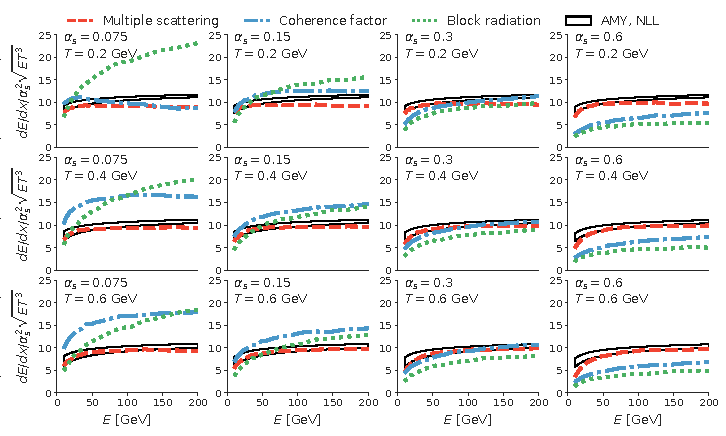
\includegraphics[width=\textwidth]{Eloss_infinite.pdf}
\caption{Energy loss per unit path lengh $dE/dx$ as a function of energy $E$, temperature $T$ and coupling constant $\alpha_s$. Each column corresponds to $\alpha_s = 0.075, 0.15, 0.3$, and $0.6$ (from left to right). Each column corresponds to $T = 0.2, 0.4$, and $0.6$ GeV (from top to bottom). $dE/dx$ is divided by the expected scaling $\alpha_s^2 \sqrt{ET^3}$. The calculations from ``Modified rescattering", ``Coherence factor", and ``Block radiation" approaches are the red-dashed lines, blue-dash-dotted lines, and green-dotted lines respectively. The AMY NLL results are denoted as black boxes.}
\label{fig:eloss-inf}
\end{figure*}

\begin{figure*}
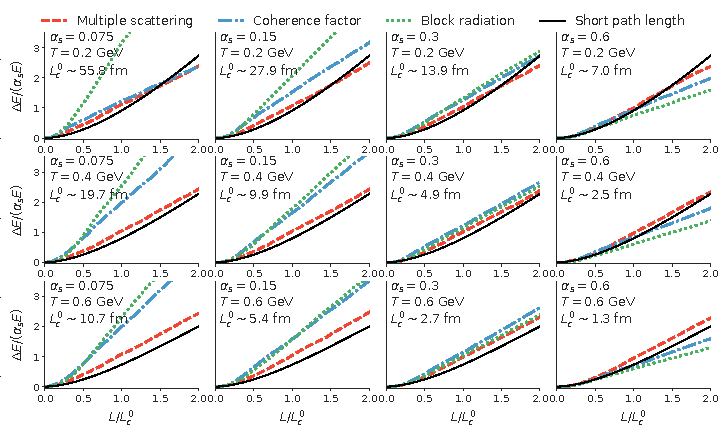
\includegraphics[width=\textwidth]{Eloss_Ldep.pdf}
\caption{Energy loss $\Delta E$ as a function of path length $L$, temperature $T$ and coupling constant $\alpha_s$. Each column corresponds to $\alpha_s = 0.075, 0.15, 0.3$, and $0.6$ (from left to right). Each column corresponds to $T = 0.2, 0.4$, and $0.6$ GeV (from top to bottom). $\Delta E$ is scaled by $\alpha_s E$ and $L$ is scaled by an estimated critical path length $L_c^0 = \sqrt{E/\hat{q}_0}$, $\hat{q}_0\sim 4\pi C_A\alpha_s^2 \times 1.28 T^3$. The calculations from ``Modified rescattering", ``Coherence factor", and ``Block radiation" approaches are the red-dashed lines, blue-dash-dotted lines, and green-dotted lines respectively. The analytic results for thin medium are denoted as black solid lines.}
\label{fig:eloss-ldep}
\end{figure*}

\begin{figure}
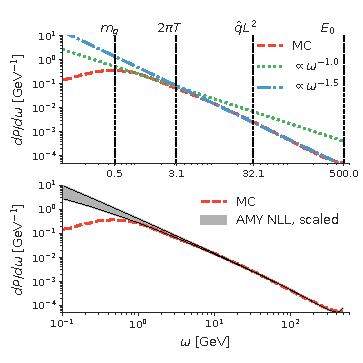
\includegraphics[width=\columnwidth]{spectrum.pdf}
\caption{Radiated gluon spectrum in an infinite medium from an energetic quark $E=500$ GeV and $\alpha_s = 0.1$. The top plot shows the spectrum (red-dashed line) and power law fit (green-dotted and blue-dash-dotted lines) in different gluon energy ($0<\omega < E$) regions, separated by the gluon thermal mass $m_g$, a thermal scale $\hat{q}_0\lambda_g^2 \sim 2\pi T$. The middle plot is the same calculation compared to incoherent spectrum and the AMY semi-analytic result. The bottom plot is the ratio between the Monte-Carlo simulation and the semi-analytic calculation.}
\label{fig:spectrum}
\end{figure}


In this section, we compare the calculations of the three different implementations described in Section \ref{section:MC} to the theoretical limits quoted and described in Section \ref{section:Theo}. 

In Figure \ref{fig:eloss-inf}. We showed the calculation of energy loss per unit path length $dE/dx$ of a quark in an ``infinitely large" medium. 
Technically, we do a time evolution long enough ($L\gg L_c$) until any finite size effect have faded away and then measure $dE/dx$.
The results presented are further divided by the anticipated scaling behavior $dE/dx \propto \alpha_s^2 \sqrt{ET^3}$.
For each column, we double the $\alpha_s$ value and for each row, temperature is increased by $0.2$ GeV. 
Within each subplot, the parton energy is varied from $10$ GeV to $200$ GeV.
Different Monte Carlo calculations are shown in colored lines, AMY NLL results are shown as black boxes. 
It is found that the ``Modified rescattering" approach (red-dashed lines) very well reproduces the energy, temperature, and coupling constant dependence of AMY NLL energy loss for relatively a high energy parton $E>20$ GeV.
For the ``Coherence factor" approach (blue-dash-dotted lines), although it does not include multiple rescatterings of the gluon. The energy dependence and temperature dependence are similar to the theoretical limits; however, it systematically deviates from the theory calculation for different coupling constant.
For the ``Blocking radiation" approaches, this $\alpha_s$-dependence deviation are even bigger and the energy dependence also gets worse, which are not surprised as we have discussed that suppression introduced in this way does not modified the shape of the spectrum.

Next we tested the path-length $L$ dependence of the energy loss $\Delta E$ of a quark with $E = 200$ GeV in a finite medium.
The comparison is showed in Figure \ref{fig:eloss-ldep}.
Again, each columns and each rows use different coupling constants and temperatures respectively and within each subplots the path length is varied up to four times of $L_c^0$.
Here $L_c^0 = \sqrt{E/\hat{q}_0}$ is an estimate of the critical path length below which a non-linear $L$-dependence is expected.
All three implementations show the non-linear path length dependence.
The ``Modified rescattering" approach stays close to the thin-medium theory calculation for $L<L_c^0$, while the other two approaches deviates systematically as $\alpha_s$ changes.

Finally, we examine the gluon radiation spectrum of a $500$ GeV quark in a $T = 0.5$ GeV infinite medium in the ``Modified Rescattering" approach, using $\alpha_s = 0.1$.
This radiation spectrum $dP/dtd\omega$ is shown in Figure \ref{fig:spectrum}. 
In the top plot, we have divided the gluon energy into different domains by the thermal mass $m_g$, and an estimate of the critical energy $\lambda_g m_D^2 \sim 2\pi T$.
The spectrum with $\omega < m_g$ is suppressed due the use of a finite mass.
In the region $m_g < \omega < 2\pi T$, the $2\rightarrow 3$ process still dominates and the spectrum follows the incoherent result using Gunion-Bertsch cross-section, scaling like $\omega^{-1}$.
Gluon with $2\pi T < \omega < E$ enters the LPM region and it should be proportional to $\omega^{-3/2}$.
The power law fitted results in each domain are very close to the expected scaling.
In the middle plot, we compare the same curve directly to the results given by incoherent rate and the semi-analytic results obtained in AMY NLL approximation. 
Their ratios are shown in the bottom plot.
The ``Modified Rescattering" approach nicely reproduce the incoherent limit with gluon thermal mass for $\omega < 2\pi T$ and the LPM suppression for $\omega > 2\pi T$. 
The percentage difference are within 15\%, this agreement is already pleasing given that we haven't fine tune the relations in Equations \ref{eq:tune} yet.

Concluding this section, we found that the ``Multiple rescattering" approach reproduce nicely the theory calculation of $dE/dx$ in an infinite medium and also has the desired energy loss scaling for a thin medium.
It grants a better theoretical control on the parton energy loss Monte Carlo which will benefit the interpretation of the result from a systematic model-to-data comparison.

\section{Expanding medium, running coupling and mass effect}\label{section:disscuss}
\begin{figure}
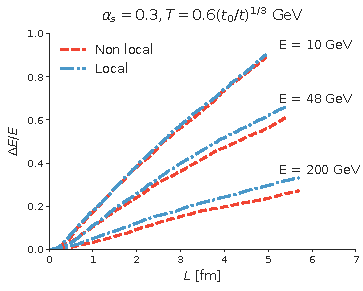
\includegraphics[width=\columnwidth]{Bjorken.pdf}
\caption{Energy loss fraction $\Delta E /E$ as function of path length $L$ at three different energies. Reddashed lines are direct simulations (the non-local case) and blue-dash-dotted lines are results using local approximation.}
\label{fig:Bjorken}
\end{figure}
Before applying this new implementation to describe energetic parton transport in heavy ion collisions, there are still a few issues we need to study and address.
The first issue concern with LPM effect in an expanding medium. 
The QGP produced in colliders only exists for a short amount of time and it undergoes violent expansion, i.e, the medium temperature may have notably changed during the formation time.
Therefore, we expect different radiation spectrum and correspondingly different amount of energy loss between the following two computing scenarios.
\begin{itemize}
\item[1.]  {\it A non-local (direct) calculation}: radiated gluons precept the changing medium within the formation times.
\item[2.] {\it A local approximation}: calculate with rates obtained in the infinite medium defined by the local temperature at the radiation vertex.
\end{itemize} 
Although a non-local scenario should be more realistic, we would like to see how close the local approximation is.
We set-up simulations in a Bjorken expansion background at mid-rapidity, and the temperature decreases with proper time,
\begin{eqnarray}
T(\Delta\tau) = T_0 \left(\frac{\tau_0}{\tau_0+\Delta\tau}\right)^{\frac{1}{3}}.
\end{eqnarray}
We chose $T_0=0.6$ GeV, $\tau_0=0.6$ fm/c and used a fixed coupling constant $\alpha_s = 0.3$.
The ``Modified rescattering" approach is already a non-local calculation. because it preforms gluon rescatterings at different space-time during the evolution. 
To mimic the local approximation, we let each pre-gluon remember the temperature where it is first created and use this local temperature to perform rescatterings.
The results are shown in Figure \ref{fig:Bjorken}. 
For low energy partons, the difference between the two scenario are negligible. The different is only moderate for a 200 GeV quark.
This is because for $\alpha_s = 0.3$ and the range of energy we considered, the maximum formation time $\sqrt{E/\hat{q}}$ is still small compared to the inverse of temperature changing rate $d\ln(T)/dt$.

\begin{figure}
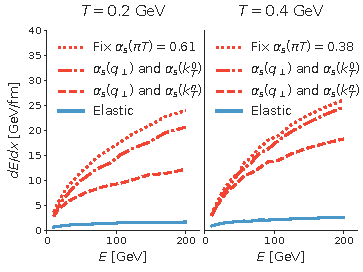
\includegraphics[width=\columnwidth]{Eloss_infinite_run.pdf}
\caption{Testing running coupling effect }
\label{fig:run}
\end{figure}
Second, we would like to improve the previous calculation with a running coupling constant. 
We followed the prescription described in [P.Arnold-2].
For each gluon elastic rescatterings, we evaluate $\alpha_s$ at the momentum transfer squared, this is already the feature in {\tt Lido} with running coupling.
The coupling constant associated to the splitting vertex is evaluated at the final gluon transverse momenta squared $k_{\perp,n}^2 = \left(\vec{k}_T^0+\vec{q}_1+\cdots+\vec{q}_n\right)^2$ because all these transverse kicks $\vec{q}_i$ add up coherently.
In the {\tt Lido} model, the original scale for this vertex is the gluon transverse momentum square in the $2\rightarrow 3$ process $k_{\perp,0}^2$.
Therefore, for the running version of this implementation, we change the acceptance probability $p$ in Step 3.2 to,
\begin{eqnarray}
p' = \min\left\{1, \frac{\tilde{\lambda}}{\tau_n}\times\frac{\alpha_s(k_{\perp,n}^2)}{\alpha_s(k_{\perp,0}^2)}\right\}
\end{eqnarray}
Because on average $k_{\perp,n}^2 \sim \hat{q}\tau_{f,n} \sim \sqrt{\hat{q}\omega}$ is larger than $k_{\perp,0}^2$, the running coupling effect reduces the radiation gluon by a factor of  $\alpha_s(k_{\perp,n}^2)/\alpha_s(k_{\perp,0}^2)$.
In Figure. \ref{fig:run}, we showed three calculations in a static medium. The dotted lines uses a fixed coupling constant evaluated at a thermal scale $2\pi T$.
This scale is also the lowest scale cut-off for the running coupling constant in our model (note that this minimum scale is not required in the original work [P.Arnold-2]).
The dash-dotted lines are running coupling calculations where the $\alpha_s(Q)$ of elastic process evaluated at $t$-channel momentum transfer and the $\alpha_s(Q^2)$ of the radiation vertex evaluated at $k_{T,0}^2$.
The dashed lines are also running coupling calculations but evaluate radiation $\alpha_s(Q^2)$ at $Q^2 = k_{\perp,n}^2$ through the modified acceptance probability $p'$.
Because the typical momenta transfer in the elastic and inelastic processes is comparable to the cut-off $Q_{\min} = 2\pi T$, the results with only the replacement $\alpha_s\rightarrow\alpha_s(q_\perp^2)$ and $\alpha_s\rightarrow\alpha_s(k_{\perp,0}^2)$ does not differ much from the fixed coupling ones.
However, the further replacement of $\alpha_s(k_{\perp,0}^2)\rightarrow\alpha_s(k_{\perp,n}^2)$ significantly reduces the amount of radiation at high energy.
We can estimated the order of magnitude o $k_{\perp,n}^2$ to be  and it is $\sqrt{\omega/T}$ times larger than the order of magnitude of $k_{\perp,0}^2$ which leads to the running coupling suppression in the expression of $p'$.

\begin{figure}
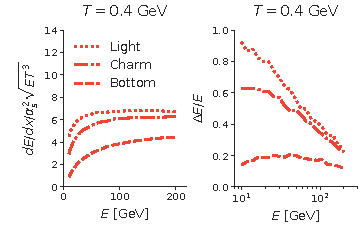
\includegraphics[width=\columnwidth]{Eloss_mass.pdf}
\caption{A demonstration of mass effect. Left plot: the scaled energy loss rate in an infinite medium for light quark, charm quark and bottom quark. Right plot: energy loss fraction of light quark, charm quark and bottom quark at path length $L=4$ fm. We used fixed coupling constant $\alpha_s(2\pi T) \approx 0.28$. }
\label{fig:mass}
\end{figure}

Finally, to apply this approach to the heavy quark sector, we put back the mass effect. 
These include the massive particle kinetics and the formation time involving a massive quark,
\begin{eqnarray}
\tau_{f} = \frac{2x(1-x)E}{k_\perp^2 + x^2M^2 + (1-x)m_g^2}.
\end{eqnarray}
Moreover, matrix-elements also need to be changed to include the so-called ``dead-cone" effect, where the collinear radiations with angles $\theta \sim k_\perp/k < M/E$ are suppressed. 
The $2\rightarrow3$ Gunion-Bertsch cross-section with mass effect has been derived [J.Uphoff], but we have shown that rescatterings increases $k_{\perp}^2$ on average, so a direct use of this massive $2\rightarrow3$ matrix-element lead to an unduly strong dead-cone effect.
The solution is to use the $2\rightarrow3$ matrix-element without mass effect to generate initial gluon, leaving the dead-cone suppression to another factor in the acceptance probability,
\begin{eqnarray}
p'' = \min\left\{1, \frac{\tilde{\lambda}}{\tau_n}\frac{\alpha_s(k_{\perp,n}^2)}{\alpha_s(k_{\perp,0}^2)} \left(\frac{k_{\perp,n}^2}{k_{\perp,n}^2+x^2 M^2}\right)^2\right\}
\end{eqnarray}
On the left of Figure \ref{fig:mass}, the scaled energy loss rate in an infinite medium is extracted from simulations for light (massless), charm ($M=1.3$ GeV) and bottom ($M=4.2$ GeV) quarks. 
On the right, it is the energy loss fraction at a finite path-length $L=4$ fm.
In both cases, the mass introduces the energy loss rate ordering, $dE_{\textrm{light}}/dx > dE_c/dx > dE_b/dx$ and the differences are smaller at high energy.


\section{Summary and outlook}\label{section:summary}
To reduces the theory uncertainty introduced in the numerical implementation of the perturbative transport approach for hard parton inside a quark-gluon plasma, we studied three different Monte-Carlo implementations and systematically compare them to the semi-analytic forms of parton energy loss.
We showed that ``Modified Rescattering" approach well reproduce the coupling constant, temperature, parton energy and path-length dependences of the theoretical calculated energy los in both infinite medium and thin medium.
It also agree with the predicted gluon spectrum within controlled uncertainty.
The non-local space-time dependence in an expanding medium only causes small to moderate change in the energy loss within interested energy range and temperature.
The running coupling effect is studied and a tentative dead-cone effect implementation is proposed.
This approach is not restricted to scattering rate based model, it also applies to a diffusion modeling of the elastic processes. 
For future studies, a control of the uncertainties between Monte-Carlo implementation and known theory calculations, a more unambiguous examination of theory assumptions and a more meaningful phenomenology extraction of jet, heavy quark transport properties can be done in the model-to-data comparisons.
Also, a Monte-Carlo that is tuned to match leading order theory calculation could be a good starting point to implement next-to-leading order corrections to the phenomenology models.


\begin{acknowledgments}
SAB and WK  are supported by the U.S. Department of Energy Grant no. DE-FG02-05ER41367. WK is also supported by NSF grant OAC-1550225.
\end{acknowledgments}

\begin{appendices}
\end{appendices}
\bibliography{mclpm} 
\end{document}